\section{Evaluation Setup}
\label{sec:eval-setup}

The evidence in this chapter comes from three sources: the automated test suite together with a static inspection of the implemented system, a set of recorded reading sessions on real hardware, and the session records those sessions export.

The reading sessions were run with a Tobii eye tracker (model \texttt{IS4\_Large\_Peripheral}) on a 2560$\times$1440 display, calibrated before each session with a nine-point screen-based procedure gated on a passing validation.
The platform runs as a single-machine deployment: the backend and both browser surfaces, the participant reader and the researcher console, executed on one host, so the traffic between each client and the backend travels over the local loopback rather than a network, which is the intended single-operator setting and the context in which the latency of \cref{sec:eval-performance} should be read.
Four participants each read an expository Markdown article under two conditions, namely with and without the context-preserving restore enabled, giving eight sessions.
\Cref{tab:eval-sessions} summarises them.
All eight sessions used the eye tracker as the sensing source, had their eye-movement analysis served by the external provider of \cref{sec:eval-modularity}, and applied typographic interventions manually through the researcher console; no automated decision strategy was active during them.
We additionally recorded one session under an advisory decision strategy, used only to exercise the decision-path instrumentation of \cref{sec:eval-performance} and kept separate from the with-and-without comparison, so the eight sessions in \cref{tab:eval-sessions} remain a clean manual-mode dataset.
The physical two-screen arrangement is shown in \cref{fig:eval-rig}.

\begin{figure}[htbp]
\centering
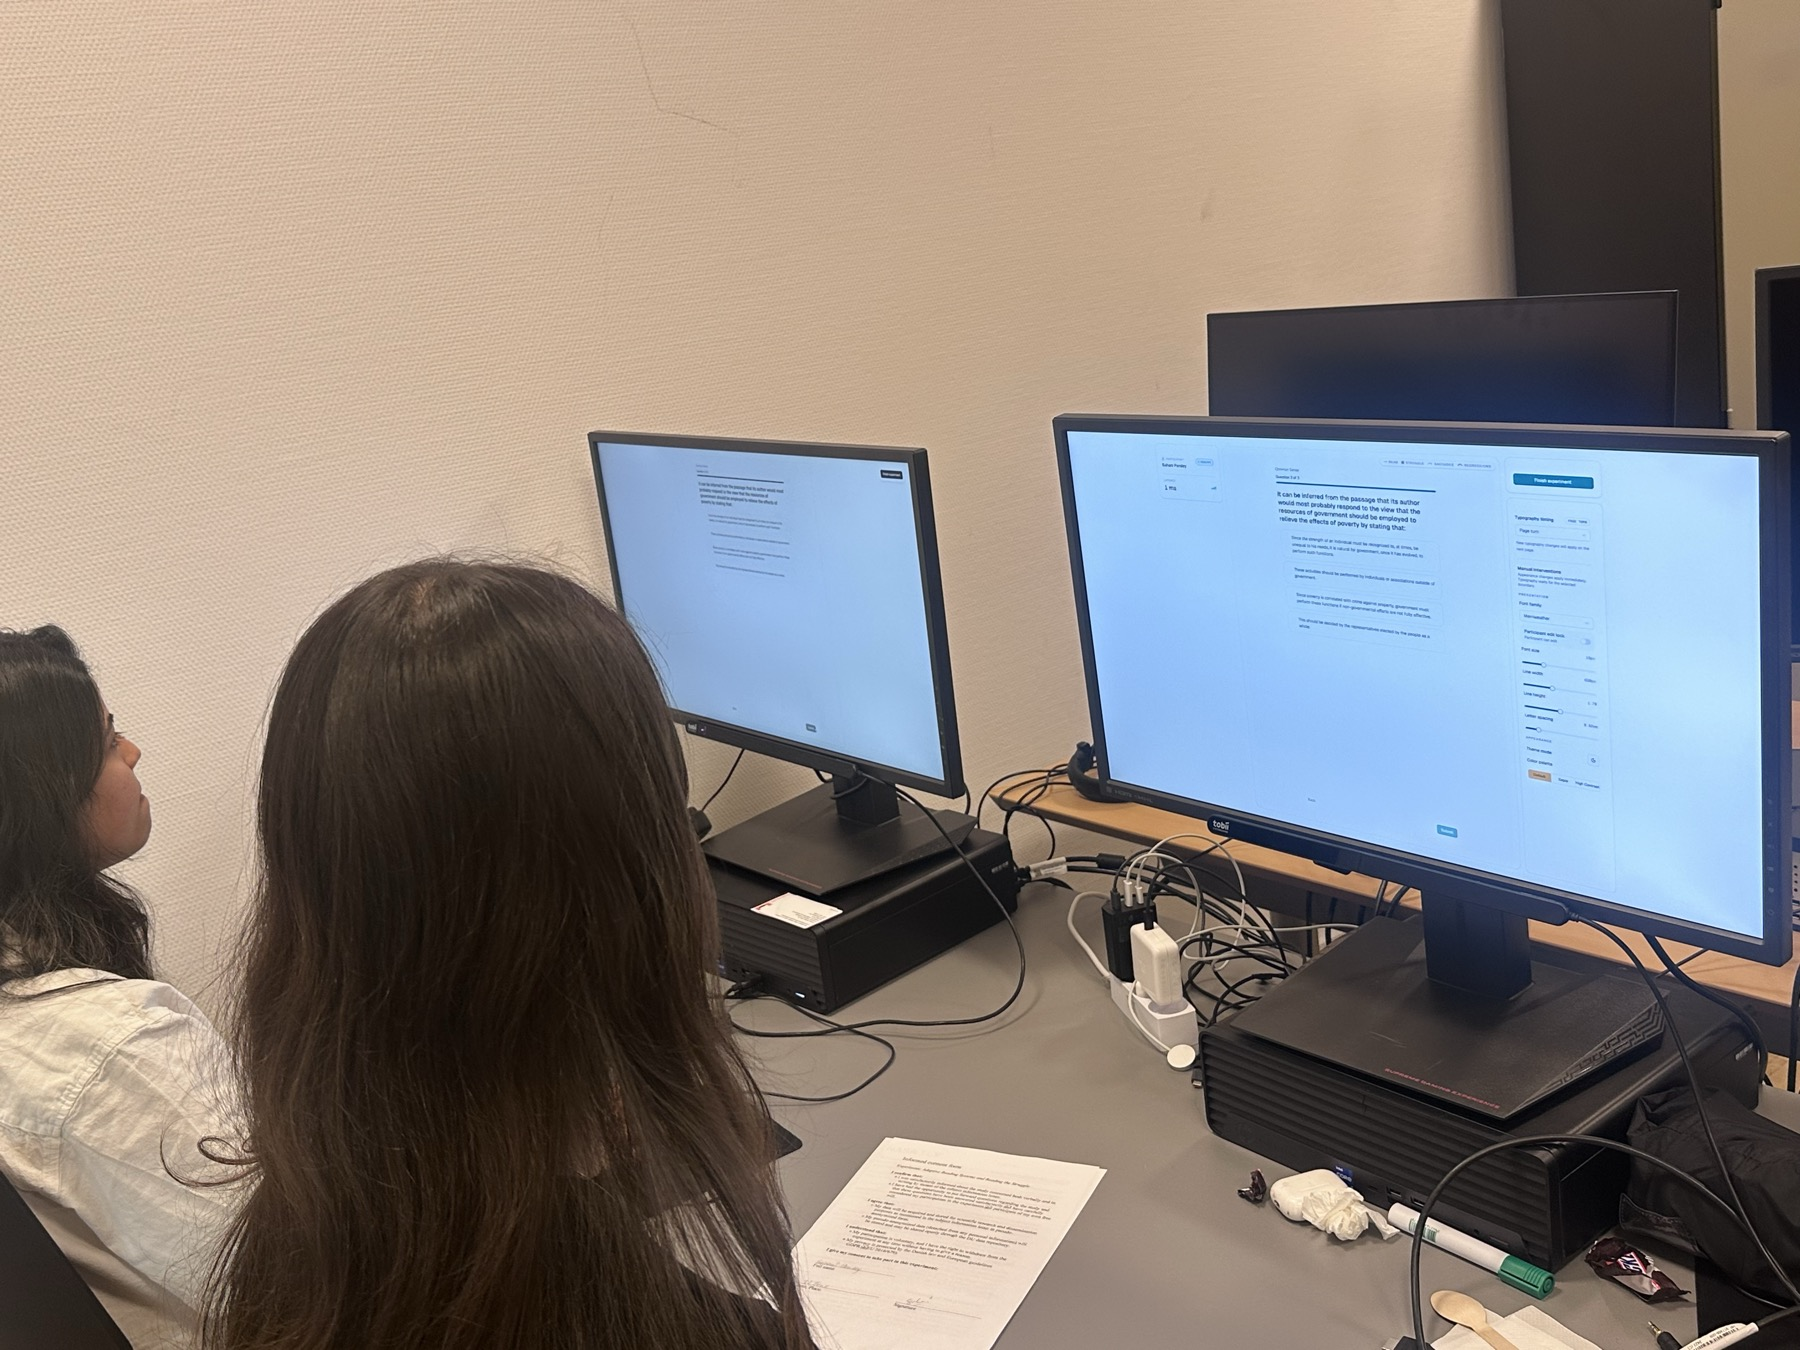
\includegraphics[width=0.82\linewidth]{Chapters/06_Implementation/experiment-setup.jpg}
\caption{The two-screen experiment setup. The participant reads the presented text on one display (left), while the researcher monitors the mirrored view and applies interventions from the console on the other (right), which carries the typographic controls; the Tobii eye tracker is mounted at the foot of the participant's display, and both surfaces are served by one backend on a single host. The participants' faces are blurred for anonymity.}
\label{fig:eval-rig}
\end{figure}

\begin{table}[htbp]
\centering
\caption{The eight recorded reading sessions that supply the runtime evidence in this chapter. Each participant read under both conditions, and the durations and counts are taken from the exported session records.}
\label{tab:eval-sessions}
\small
\begin{tabular}{llrrrr}
\toprule
Participant & Condition & Duration (s) & Gaze samples & Fixations & Interventions \\
\midrule
P1 & With preservation    & 186 & 16664 & 656  & 5 \\
P2 & With preservation    & 252 & 22688 & 1525 & 7 \\
P3 & With preservation    & 171 & 15305 & 866  & 3 \\
P4 & With preservation    & 224 & 20136 & 943  & 4 \\
P1 & Without preservation & 475 & 42683 & 1914 & 9 \\
P2 & Without preservation & 123 & 11063 & 719  & 4 \\
P3 & Without preservation & 386 & 34624 & 1994 & 11 \\
P4 & Without preservation & 141 & 12697 & 694  & 2 \\
\bottomrule
\end{tabular}
\end{table}

Every session is exported as a schema-versioned record together with a separate telemetry record, and the analysis that produces the figures and tables below reads only those exported files.
The analysis pipeline is scripted and re-runnable, so each figure traces to a recorded session rather than to a live observation.
We make no inferential claim from these sessions: with four participants the behavioural numbers in \cref{sec:eval-context} are descriptive, consistent with the scope set out in \cref{sec:final-problem-statement}, which places a controlled human-subjects effect study outside this thesis.
